\documentclass[12pt]{article}
\usepackage[top=1in,bottom=1in,left=1in,right=1in]{geometry}
\usepackage{alltt}
\usepackage{array}	
\usepackage{graphicx}
\usepackage{tabularx}
\usepackage{verbatim}
\usepackage{setspace}
\usepackage{listings}
\usepackage{amssymb,amsmath, amsthm}
\usepackage{qtree}
\usepackage{hyperref}
\usepackage{oz}
\usepackage[cc]{titlepic}
\usepackage{fancyvrb}
\usepackage{epstopdf}
\usepackage{soul}
\usepackage{array}
\usepackage{graphicx}
\graphicspath{ {./images/} }
\newcolumntype{L}{>{\centering\arraybackslash}m{3cm}}
\usepackage[affil-it]{authblk}

% title
\title{SOEN 331: Introduction to Formal Methods for Software Engineering \\ \\
\textbf{Assignment 1} \\ \\
Propositional and Predicate Logic, Structures,\\Binary Relations, Functions, Orderings and Construction Techniques}

 \affil{Gina Cody School of Computer Science and Software Engineering \\
    Concordia University, Montreal, QC, Canada}
\date{Winter 2024}

\begin{document}
\maketitle

\newpage
\tableofcontents
\newpage


\newpage

\section{Problem 1 (5 pts)}

\subsection{Answer:}

Assume that p represents the statement "The face of a card is \textbf{blue}" and  q represent "It has a \textbf{prime} on the other side". The proposition could be expressed as p $\rightarrow$ q  \\ \\
We must turn over the card shows the color \textbf{blue}, and expect to see prime. Because this card shows the color blue, to validate the truth of the proposition, this card must be turned over and check if its back has a prime number. In other words, the statement p is true. In order to validate the proposition p $\rightarrow$ q, q has to be true. Therefore the turned card's back is expected to have prime number. \\ \\
Taking the contrapositive of the implication statement, $\neg q $\rightarrow$ \neg p$ ($\neg prime $\rightarrow$ \neg blue$). We must turn over the card shows number \textbf{9} - not a prime number, and expect to not see blue color in the back, in this case, we expect to see yellow. \\ \\
We cannot make any claim based on the card shows number \textbf{11}. In this case, the statement q is true, the card has prime number). The proposition p $\rightarrow$ q will be true regardless the truth value of p - the another side of the card could be blue or yellow. \\ \\
We cannot make any claim based on the card shows \textbf{yellow}. Because the statement p is false in this case ($\neg blue$), as this card has yellow color on one side. Therefore, no matter the back of the card is prime or not prime, this will not affect the truth of the proposition. \\ \\
In conclusion, the cards with visible sides blue and 9 must be turned over.


\newpage

\section{Problem 2 (14 pts)}

\subsection{Part 1}
\begin{enumerate}
\item Construct a formula in predicate logic to define a planet, where planet is defined
as an object whose mass is greater than $0.33 \times 10^{24}KG$, and which it orbits around the
sun. For all practical purposes, you may ignore the $10^{24}KG$ factor.\\

Formula for Planet:
\[\textit{Planet}(\textit{object}) \equiv \exists \textit{mass} \left( \textit{Mass}(\textit{object}, \textit{mass}) \land \textit{mass} > 0.33 \right) \land \textit{Orbits}(\textit{object}, \textit{sun})\]

Formula for \textit{is\_sattelite\_of}:
\[\textit{is\_sattelite\_of} \equiv \textit{Orbits}(\textit{sattelite}, \textit{object}) \land \textit{Planet}(\textit{object})\]
\\
\item Map your formulas to Prolog rules is planet/1, and is satellite of/2, and demonstrate how it works by executing both ground- and non-ground queries. Identify the type of each query.

Here we have the 2 main rules \textit{is\_planet} and
\textit{is\_satellite\_of}. 
    \begin{lstlisting}
    
        is_planet(P) :-
            object(P),
            mass(P, Mass),
            Mass >= 0.33,
            orbits(P, sun).

            
        is_satellite_of(S, P) :-
            object(S),
            is_planet(P),
            orbits(S, P).

            
    \end{lstlisting}

Below you can see the interaction with the Prolog interpreter(to be able to see the multiple results, you need to press \textit{space}).
    \begin{figure}[hbt!]
        \centering
        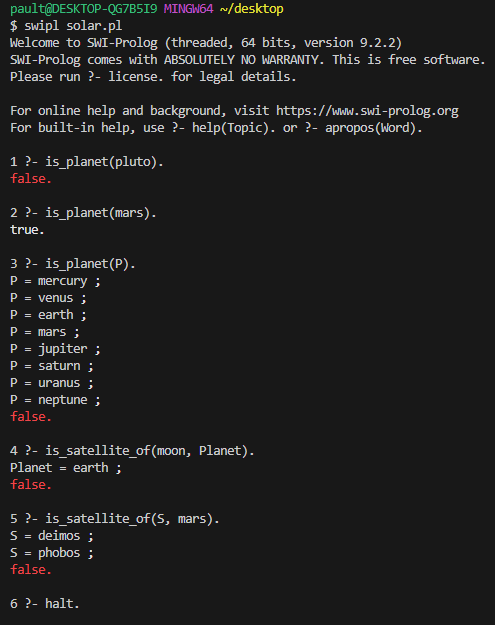
\includegraphics[scale=0.5]{assigment1/331A1_num2_part2.png}
        \caption{Prolog interaction for problem 2 part 2}
    \end{figure}\\
\newpage    
\item Construct a Prolog rule obtain all satellites/2 that succeeds by returning a collection of all satellites of a given planet.

Here we have the 2 main rules \textit{is\_planet} and \textit{is\_satellite\_of}.    
    \begin{lstlisting}
        is_planet(P) :-
            object(P),
            mass(P, Mass),
            Mass >= 0.33,
            orbits(P, sun).

        is_satellite_of(S, P) :-
            object(S),
            is_planet(P),
            orbits(S, P).
    \end{lstlisting}

    \begin{lstlisting}
        obtain_all_satellites(Planet, Satellites) :-
            findall(Satellite, is_satellite_of(Satellite, Planet)
            , Satellites).
    \end{lstlisting} \\
    \begin{figure}[hbt!]
        \centering
        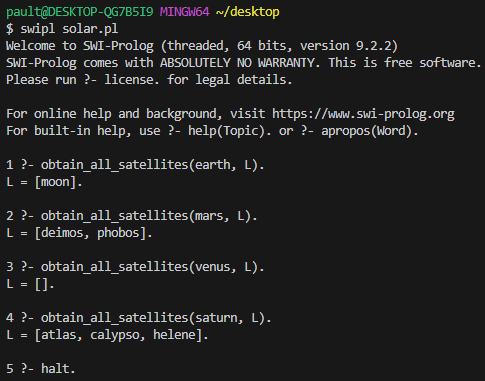
\includegraphics[scale=0.6]{assigment1/331A1_num2_part3.png}
        \caption{Prolog interaction for problem 2 part 3}
    \end{figure}\\

\end{enumerate}


\newpage

\subsection{Part 2: Categorical propositions}
\begin{enumerate}
    \item "Some numbers are not composite"\\
    \underline{Answer:}\\
    This is: $\exists x(number(x) \wedge \neg composite(x))$. Type  O.
    \\
    \item "No numbers are prime"\\
    \underline{Answer:}\\
    Rephrased as: "All numbers are composite". $\forall x(number(x) \wedge composite(x))$. Type A.
    \\
    \item "Some numbers are not prime"\\
    \underline{Answer:}\\
    Rephrased as: "Some numbers are composite". $\exists x(number(x) \wedge composite(x))$. Type I.
    \\
    \item "All numbers are prime"\\
    \underline{Answer:}\\
    Rephrased as: "No numbers are composite". $\forall x(number(x) \wedge \neg composite(x))$. Type E.
    \\
\end{enumerate}
\newpage
\subsection{Part 3: Categorical propositions}
\begin{enumerate}
    \item Prove formally that negating A is logically equivalent to obtaining O (and vice versa).\\ \\
Let A be the statement $\forall$ s : S \mid (s $\in$ P).\\
The negation of A, $\neg$A is $\neg(\forall$ s : S \mid (s $\in$ P)).\\
By De Morgan's, $\neg$A is equivalent to $\exists$ s : S \mid ($\neg$ (s $\in$ P)).\\
Therefore, negating A yields \textit{O}, since $\exists$ s : S \mid ($\neg$ (s $\in$ P)) is the definition of an \textit{O} proposition.

    \item Prove formally that negating E is logically equivalent to obtaining I (and vice versa).\\ \\
Let E be the statement $\neg(\exists$ s : S (s $\in$ P)).\\
The negation of E, $\neg$E is $\neg(\neg(\exists$ s : S (s $\in$ P))).\\
By the law of double negation, $\neg$E is equivalent to $\exists$ s : S (s $\in$ P).\\
Therefore, negating E yields \textit{I}, since $\exists$ s : S (s $\in$ P) is the definition of an \textit{I} proposition.


\end{enumerate}
\clearpage
\newpage

\section{Problem 3 (22 pts)}

\subsection{Part 1}
\begin{enumerate}
    \item Visualize all models of behavior.
    \begin{figure}[hbt!]
        \centering
        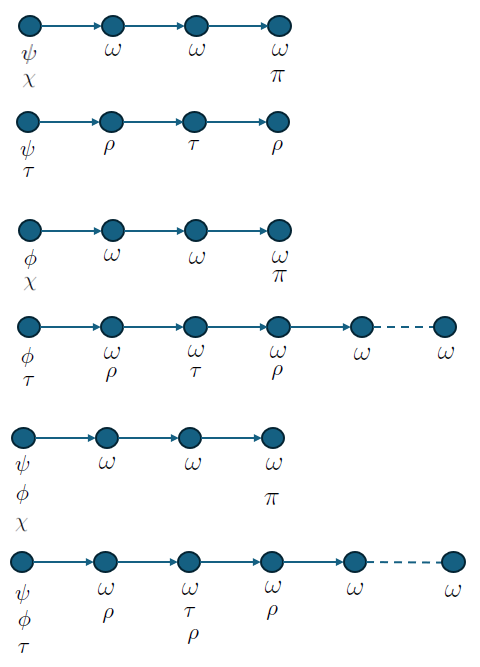
\includegraphics[scale=0.6]{assigment1/331A1_num3_part1.png}
        \caption{Models of behavior for Problem 3.1.1}
        \label{fig:model_behavior}
    \end{figure}

    \item Make observations on the visualization by specifying exact conditions about
termination, non-termination and consistency (or lack thereof), if any exist.\\

\textbf{Termination: } A you can see with the image above, we have some models that will terminate. For example, the first one will terminate because as soon as $\pi$ is true, the other condition ($\pi\mathcal{R}\omega$) will stop.\\ \\
\textbf{Non-termination: } The examples 4 and 6 represent non-termination models since $\omega$ will stay true until and including the state at which $\pi$ first becomes true.\\ \\
\textbf{Consistency: } They are not paths that are consistent with the temporal formula. The closest one is the last one that adheres to 6 out of the 7 of the temporal constraints.\\ \\

\end{enumerate}

\subsection{Part 2}
\begin{enumerate}
    \item Formalize and visualize the following requirement: “If none of ϕ or ψ are
invariants, then starting from time = i + 2, χ will eventually become true and it will
remain true up to and including the moment τ first becomes true. Note that there
exists no guarantee that τ ever becomes true.”
    \begin{figure}[hbt!]
        \centering
        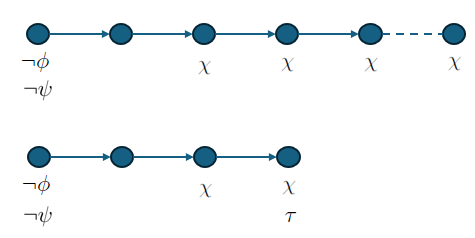
\includegraphics[scale=0.58]{assigment1/331A1_num3_part2.1.png}
        \caption{Models of behavior for Problem 3.2.1}
        \label{fig:model_behavior}
    \end{figure}

\begin{lstlsting}

This requirement can be formalize as follows:\[
    (\neg\phi \vee \neg\psi) \rightarrow \bigcirc^2(\Box \chi \land (\chi \mathcal{U} \tau))
    \]

    \item Describe the visualize the following requirement: \[
    (\neg\alpha \vee \neg\beta) \rightarrow (\bigcirc\diamond(\gamma \mathcal{U} \delta))
    \]

($\neg \alpha \land \neg \beta$) signifies that either $\alpha$ is not true, or  $\beta$ is not true, or both are not true. $(\bigcirc\diamond(\gamma \mathcal{U} \delta))$ means that there will eventually be a time from which point forward ($\Box$) it will always be the case that $\gamma$ holds until $\delta$ becomes true. Note that in this case, $\delta$ is guaranteed to become true at some future time. This is the definition of the $\mathcal{U}$ operation.
    \begin{figure}[hbt!]
        \centering
        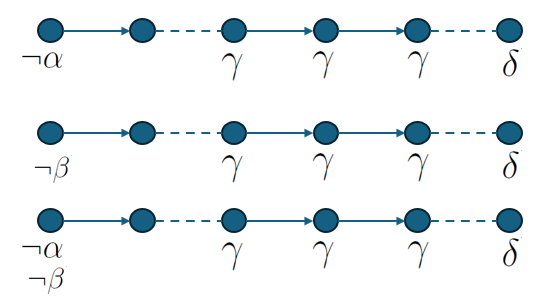
\includegraphics[scale=0.5]{assigment1/331A1_num3_part2.2.png}
        \caption{Models of behavior for Problem 3.2.2}
        \label{fig:model_behavior}
    \end{figure}

    \item Describe the visualize the following requirement: \[
    (\bigcirc \tau \land \bigcirc \Box \Diamond \chi) \rightarrow \bigcirc^2 (\phi \mathcal{W} \psi)
    \]
This requirement signifies that at iteration \textit{i + 1} $\tau$ will become true and eventually $\chi$ will always be true (not necessarily at \textit{i + 1}). At \textit{i + 2} $\psi$ will be true until $\phi$ becomes true.
    \begin{figure}[hbt!]
        \centering
        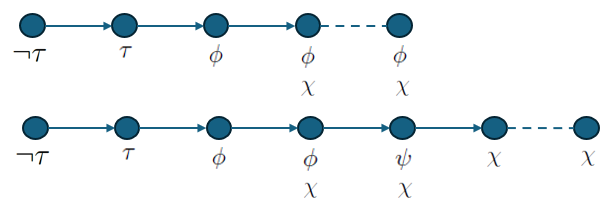
\includegraphics[scale=0.5]{assigment1/331A1_num3_part2.3.png}
        \caption{Models of behavior for Problem 3.2.3}
        \label{fig:model_behavior}\\
    \end{figure}

\end{enumerate}

\newpage

\section{Problem 4 (14 pts)}
\begin{enumerate}
    \item Provide a description (in plain English) on what is meant by $\textit{\mathcal{P} Languages}:$\\ \\
    $\textit{\mathcal{P} Languages} $ is the power set of \textit{Languages} set, which contains all subsets of the given set. In this case, it contains all subsets of \textit{Languages} set.
    \item Describe in detail (a) what the expression $\textit{Favourites: \mathcal{P} Languages}$ signifies and (b) how it should be interpreted. (c) What could be any legitimate value for variable Favorites?\\ \\
    This expression is a \textbf{variable declaration}, in which the LHS specifies a variable and the RHS defines a type.
    In this case, this expression can be expressed as "The variable \textit{Favourites} can assume any value supported by the power set of \textit{Languages}. It means any subset that can be produced from set \textit{Languages} can be a legitimate value of \textit{Favourites}.
    \item What does the expression \textit{Favourites} = \textit{P Languages} signify and (b) Is semantically equivalent to $\textit{Favourites: \mathcal{P} Languages}$\\ \\
    This expression is an \textbf{assignment statement}, it assigns the value of the RHS (which is a set) to the variable on the LHS. In this case, variable \textit{Favourites} is assigned to the power set of \textit{Languages}. Meanwhile, in the variable declaration, a variable is associated to a type. Therefore, the two expressions are \textit{not semantically equivalent}.
    \item Is $\{ \textit{Lua, Groovy, C} \}$ $\in \textit{P Languages}$? Explain in detail.\\ \\ 
    No, because \{\textit{Lua, Groovy, C}\} is not an element of the power set \textit{P Languages}.
    \item Is $\{\{ \textit{Lua, Groovy, C} \}\}$ $\subset \textit{P Languages}$? Explain in detail.\\ \\ 
    Yes, because \{\{\textit{Lua, Groovy, C}\}\} is a set of sets.
    \item What is the difference between the following two variable declarations (\textit{Languages, P Languages}) and are the two variables atomic and non-atomic? \\ \\
    \textit{Languages} is a variable, it is a set contains atomic variables and another set. Therefore, it is non-atomic.\\
    \textit{P Languages} is the power set of \textit{Languages} set, it contains all of the subsets of the given set. Therefore, it is also non-atomic. 
    \item In the expression \textit{Library} = \{\textit{C, Ruby, Go}\}, where the variable is used to hold any collection that can be constructed from \textit{Languages}, what is the type of the variable?\\ \\
    The variable \textit{Library} is a \textbf{composite}. It is a set.
    \item Is $\{\emptyset\} \in \textit{P Languages}$? Explain.\\ \\ 
    No, There is no set that contains the empty set in the power set of \textit{Languages}.
    \item \textbf{Programming} using Commom LISP\\ \\
    Common Lisp contains some build-in functions such as: \\\\
    \textbf{member item list: } returns true if item is an element of list. Otherwise, it returns false.\\
    \textbf{equal obj1 obj2: } returns true if two objects are equal. Otherwise, it returns false.
    Using the given build-in functions, the implementation using Common Lisp is as follows: 
    \begin{lstlisting}
        (defun is-memberp (set1 set2)
            (if (null set 1)
            t
            (if (member (car set1) set2)
                (is-memberp (cdr set1) set2)
            nil
            )
            ))
    \end{lstlisting}\\ \\
    \begin{lstlisting}
        (defun equal-setsp (set1 set2)
            (and (is-memberp set1 set2) (is-memberp set2 set1)))
    \end{lstlisting}\\ \\
    Example runs are as follows: \\\\
    $\mathbb{>}$ (is-memberp '() '(a, b, c, d))\\
    T\\
    $\mathbb{>}$ (is-memberp '(a, c) '(a, b, c, d))\\
    T\\
    $\mathbb{>}$ (is-memberp '(a, e) '(a, b, c, d))\\
    NIL\\
    $\mathbb{>}$ (is-memberp '(a, d) '(a, b, c, d))\\
    T\\ \\
    $\mathbb{>}$ (equal-setsp '() '(a, b, c, d))\\
    NIL\\
    $\mathbb{>}$ (equal-setsp '(a, b, c) '(a, c, b))\\
    T\\
    $\mathbb{>}$ (equal-setsp '(a, b) '(a, b, c, d))\\
    NIL\\
    $\mathbb{>}$ (equal-setsp '() '())\\
    T\\
    
    
    
\end{enumerate}

\newpage


\lstset{
  escapeinside={(*}{*)},
}
\section{Problem 5 (15 pts)}
\begin{enumerate}
    \item Define operations \textit{Enqueue}($\mathscr{Q}, \mathscr{T}$) and \textit{Dequeue}($\mathscr{Q}$).\\
    \begin{itemize}
        \item \textit{Enqueue}($\mathscr{Q}, \mathscr{T}$) is an operation that is used to insert an element to the rear end of the queue. In this case, the queue ADT is defined using two stack $\Sigma_{1}$ and $\Sigma_{2}$. In order to implement the enqueue operation, it can use the push() operation of the Stack ADT to complete. In addition, the Stack ADT is implemented using List $\Lambda$, so the push() operation could be implemented using the cons() operation of the List $\Lambda$, it adds an element at the top of the Stack. Therefore, using cons() operation of the List to implement push() operation of Stack, and then implement Enqueue() operation of Queue ADT. This allows to insert an element at the rear end of the queue (enqueue).\\ \\
        \begin{lstlisting}
            push((*$\Lambda$*), T) is
                cons(T, (*$\Lambda$*))
                
            enqueue(Q, T) is
                push(Q, T)
        \end{lstlisting}
        
        \item \textit{Dequeue}($\mathscr{Q}$) is an operation of Queue ADT that removes an element from the front end of the queue. Because the Queue ADT is implemented using two Stacks $\Sigma_{1}$ and $\Sigma_{2}$, the elements will be moved from a stack to another stack, e.g from $\Sigma_{1}$ to $\Sigma_{2}$, by using push() operation to gradually add to the top of $\Sigma_{2}$ the element of the top of $\Sigma_{1}$. Eventually, the top of $\Sigma_{2}$ is the front end of the Queue ADT. Then this front end can be removed using pop() operation of Stack, in which this pop() operation is implemented using head() and tail() operations (car, cdr).\\ \\
        \begin{lstlisting}[mathscape]
            pop(stack) is
                if not(isEmpty((*$\Lambda$*)))
                    el = g()
                    (*$\Lambda$*)' = f((*$\Lambda$*))
                return el

            dequeue(Q)
                if (isEmpty((*$\Sigma_{1}$*)) && isEmpty((*$\Sigma_{2}$*)) )
                    nil
                if (isEmpty((*$\Sigma_{2}$*)))
                    while(not(isEmpty((*$\Sigma_{1}$*))))
                        push((*$\Sigma_{2}$*), pop((*$\Sigma_{1}$*)))
                return pop(((*$\Sigma_{2}$*)))
        \end{lstlisting}
    \end{itemize}



    \item Use Common LISP to define two stacks (\texttt{stack1} and
\texttt{stack2}) as global variables to hold the collection, and implement functions \texttt{enqueue}
and \texttt{dequeue}. Place your code in file \texttt{queue-adt.lisp}, and include your interaction
with the language environment to demonstrate the behavior of your code.\\ \\
The Code for the implementations of Enqueue and Dequeue: 
\begin{lstlisting}
(defun push (stack element)
  (cons element stack))

(defun pop (stack)
  (if (null stack)
      (error "Stack is empty")
      (values (car stack) (cdr stack))))

(defun stack-empty? (stack)
  (null stack))

(defun enqueue (queue element)
  (setf (symbol-value 's1) (push (symbol-value 's1) element)))

(defun dequeue (queue)
  (if (stack-empty? (symbol-value 's2))
      (progn
        (while (not (stack-empty? (symbol-value 's1)))
          (multiple-value-bind (element remaining-stack) 
          (pop (symbol-value 's1))
            (setf (symbol-value 's2) 
            (push (symbol-value 's2) element))))
        (if (stack-empty? (symbol-value 's2))
            (error "Queue is empty")))
      nil)
  (multiple-value-bind (element remaining-stack) 
  (pop (symbol-value 's2))
    (setf (symbol-value 's2) remaining-stack)
    element))
\end{lstlisting}
\newpage
The interation with Queue ADT: \\ \\ 

(setq s1 nil) ;Initialize $\Sigma_1$ stack \\
(setq s2 nil) ;Initialize $\Sigma_2$ Stack \\

(enqueue 'q 'a)\\
(enqueue 'q 'b)\\
(enqueue 'q 'c)\\\\
(print (dequeue 'q))\\
$\mathbb{>}$A\\
(print (dequeue 'q))\\
$\mathbb{>}$B\\
(print (dequeue 'q))\\
$\mathbb{>}$C\\

    \item Implement operations \textit{head}, \textit{tail} and \textit{cons} in Prolog and demonstrate their usage (include your interaction with the language environment in your submission).
\\
    \begin{figure}[hbt!]
        \centering
        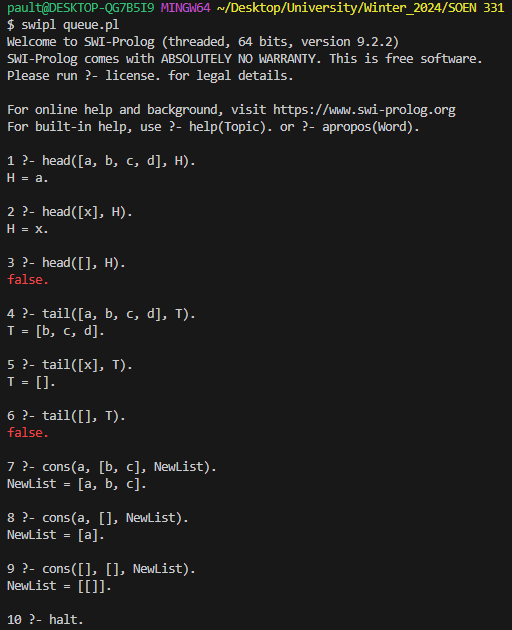
\includegraphics[scale=0.6]{assigment1/331A1_num5_part3.png}
        \caption{Prolog interaction for problem 5 part 3}
    \end{figure}
    
\end{enumerate}
\clearpage
\newpage

\section{Problem 6 (20 pts)}

\subsection{Part 1:}
\begin{enumerate}
    \item In order to prove that the binary relation R: \textit{"is of type"} in the domain of types in the Java API is \textit{a partial order}, it is necessary to prove that binary relation R satisfies three properties: reflexivity, antisymmetry, and transitivity. Consider set A is the domain of types in the Java API.
    \begin{itemize}
        \item \textbf{Reflexivity: } When $\forall a \in$ A: aRa. In this case, for any type a in A, a is type of a. This is true since every type is inherently of its own type.
        \item \textbf{Antisymmetry: } When $\forall a, b \in A: (aRb \wedge bRa) \rightarrow a = b$. If a is of type b and b is of type a, then a must be equal to b. This property is satisfied as in Java, two types are of type to each other only if they are equal. 
        \item \textbf{Transitivity: } When $\forall a, b, c \in A: (aRb \wedge bRc) \rightarrow aRc$. If type a is type of b and type b is type of c, then type a is type of c. This property is true because if a class or interface or extends another type, and that type implements of extends another type (is type of another type), then the first type is also of the last type. \\ \\
        Therefore, the binary relation R is a partial order as it satisfies three properties: reflexivity, antisymmetry, and transitivity. 
    \end{itemize}
    \item To prove ($V_{1}$, R) is a poset, it is neccessary to procve that the binary relation R is a partial order over $V_{1}$. It means that the relation must satisfy three properties: reflexivity, antisymmetry, transitivity. 
    \begin{itemize}
        \item \textbf{Reflexivity: } When $\forall a \in$ $V_{1}$: aRa. In this case, for any type a in $V_{1}$, a is type of a. This is true since every type is of its own type. Which means that the provided edges have self-loops.
        \item \textbf{Antisymmetry: } When $\forall a, b \in V_{1}: (aRb \wedge bRa) \rightarrow a = b$. If a is of type b and b is of type a, then a must be equal to b. From the provided edges, it is observed that there are no two different vertices a, b such that aRb and bRa hold. E.g: There are no (HashMap, AbstractMap) and (AbstractMap, HashMap) hold. Therefore, antisymmetry is satisfied.
        \item \textbf{Transitivity: } When $\forall a, b, c \in V_{1}: (aRb \wedge bRc) \rightarrow aRc$. If type a is type of b and type b is type of c, then type a is type of c. According to the provided edges, there are no vertices a, b,c such that aRb and bRc. E.g: There are no sets of edges such that (LinkedHashMap, HashMap), (HashMap, AbstractMap), and (LinkedHashMap, AbstractMap). Therefore, the relation is transitive.\\ \\
        Therefore, ($V_{1}$, R) is a poset as it satisfies three properties: reflexivity, antisymmetry, and transitivity. 
    \end{itemize}
    \item Hasse Diagram \\
    \begin{figure}[hbt!]
        \centering
        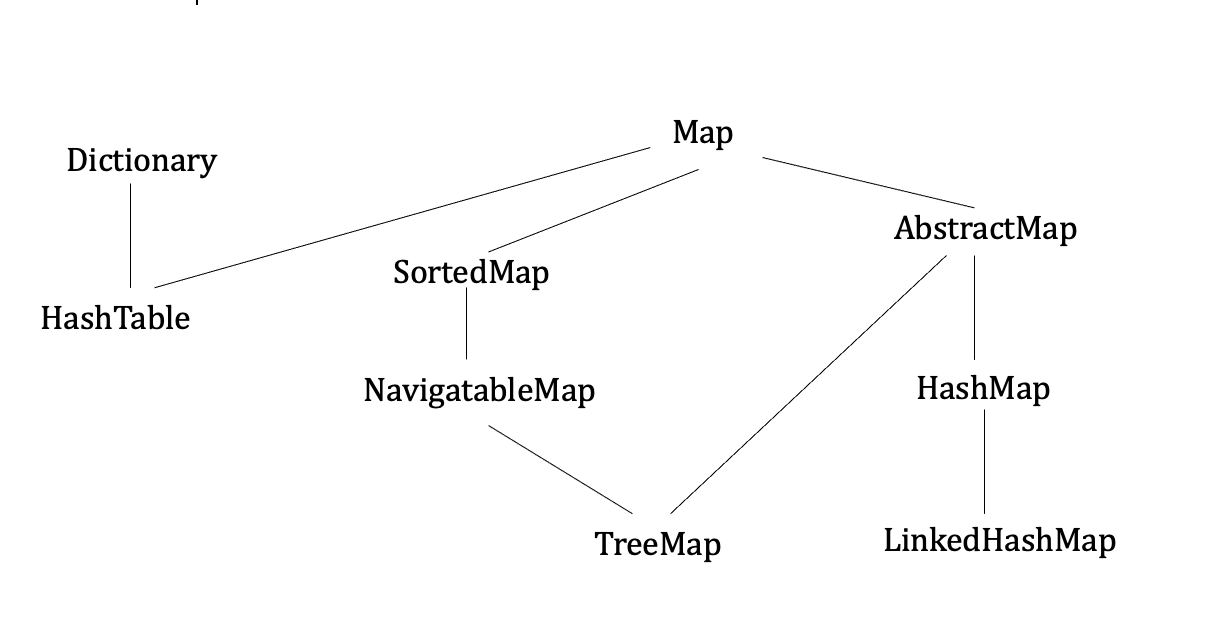
\includegraphics[scale=0.5]{HasseProblem613.png}
        \caption{Hasse Diagram for Problem 6.1.3}
        \label{fig:Hasse613}
    \end{figure}\\
    From Figure \ref{fig:Hasse613}, there is three minimal elements (HashTable, TreeMap, and LinkedHashMap), and two maximal elements (Dictionary, Map).
\end{enumerate}
\subsection{Part 2:}
\begin{enumerate}
    \item To prove that $\subseteq$ (is subset of) is a partial order, it is needed to indicate that $\subseteq$ satisfies three properties: reflexivity, antisymmetry, and transitivity. Consider A is the domain of sets.
    \begin{itemize}
        \item \textbf{Reflexivity: } When $\forall a \in$ A: a$\subseteq$a. This property is satisfied since every set is a subset of itself.    
        \item \textbf{Antisymmetry: } When $\forall a, b \in A: (a$\subseteq$b \wedge b$\subseteq$a) \rightarrow a = b$. This property is true because if two sets are subsets of each other, they must be equal.
        \item \textbf{Transitivity:} When $\forall a, b, c \in A: (a\subseteq b \wedge b\subseteq c) \rightarrow a\subseteq c$. This property holds its validity, because if a is a subset of b and b is a subset of c, a is a subset of c. \\ \\
        Therefore, $\subseteq$ is a partial order as it satisfies three properties: reflexivity, antisymmetry, transitivity.
    \end{itemize}
    \item \textit{P}($V_{2}$) is the power set of $V_{2}$ = \{a, b, c\}. This is the set containing all subsets of the set $V_{2}$. It is define as follows:\\ \\
    $\textit{P}\{a, b, c\} = \\
    \{ \\
    \emptyset, \\
    \{a\}, \{b\}, \{c\},\\
    \{a, b\}, \{a, c\}, \{b, c\},\\
    \{a, b, c\}\\
    \}\\ \\$
    To prove that ($\textit{P}(V_{2}), \subseteq$) is a poset, it is required to prove that the binary relation $\subseteq$ is a partial order over the power set \textit{P}. It means that the binary relation $\subseteq$ must satisfy three properties: reflexivity, antisymmetry, transitivity.
    \begin{itemize}
        \item \textbf{Reflexivity: } When $\forall a \in$ P: a$\subseteq$a. This property is satisfied because for every subset in P, it is a subset of itself. 
        \item \textbf{Antisymmetry: } When $\forall a, b \in P: (a$\subseteq$b \wedge  b$\subseteq$a) \rightarrow a = b$. This property is true because if two sets are subsets of each other, they must be equal. In this case, it is observed that there are not two subsets such as \{a, b\}, \{b, a\} in P. Therefore, this property is true.
        \item \textbf{Transitivity:} When $\forall a, b, c \in P: (a\subseteq b \wedge b\subseteq c) \rightarrow a\subseteq c$. This property is true, because if a is a subset of b and b is a subset of c, a is a subset of c. E.g: \{a\} is a subset of \{a, b\}, and \{a, b\} is a subset of \{a, b, c\}, then \{a\} is a subset of \{a, b, c\}. \{a\}, \{a, b\}, \{a, b, c\} are subsets of P. \\ \\
        Therefore, ($\textit{P}(V_{2}), \subseteq$) is a poset as it satisfies three properties: reflexivity, antisymmetry, transitivity. 
    \end{itemize}
    \item Hasse Diagram \\
    \begin{figure}[hbt!]
        \centering
        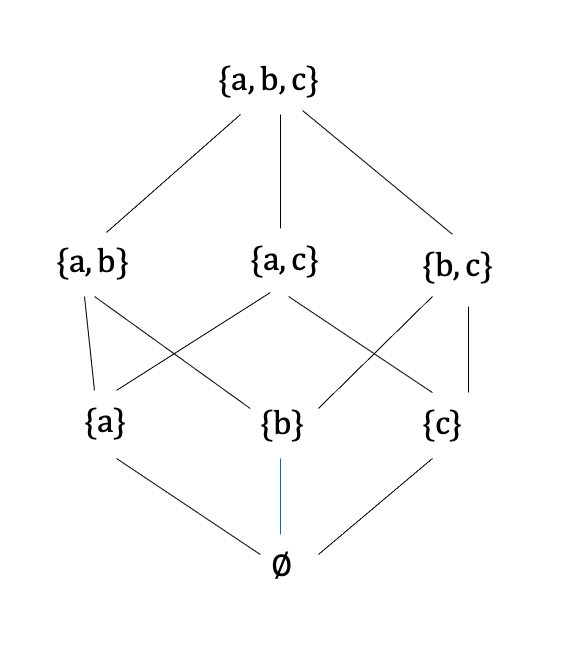
\includegraphics[scale=0.5]{HasseProblem63.png}
        \caption{Hasse Diagram for Problem 6.2.3}
        \label{fig:Hasse63}
    \end{figure}\\
    From Figure \ref{fig:Hasse63} There is one minimal element, $\emptyset$ and one maximal element, \{a, b, c\}.

\end{enumerate}
\subsection{Part 3: }
\textbf{Mapping: }Mapping map is a \textit{partial function} as it is a function defined for some subset of $V_{1}$. It does not force the mapping of every element of $V_{1}$ to an element of $\textit{P}(V_{2})$\\ \\
\textbf{Injectivity: }The function is not injective because it does not satisfy the condition of injectivity such that $\forall a, b (a \neq b \rightarrow f(a) \neq f(b))$. In this case, Dictionary and AbstractMap are mapped to the same element (\{a, b, c\}). \\ \\
\textbf{Surjectivity: }The fucntion is surjective as it is the case that $\forall b \exists a (f(a) = b)$. It can be observed that for each element of the codomain, it is mapped with at least one element in the domain. \\ \\
\textbf{Bijection: }By definition, the function is not bijective as it is not the case that both injectivity and surjectivity are satisfied. \\ \\ 
\textbf{Order preserving: }This function is not order-preserving as it is not the case that x $\prec$ y in domain of map, implies f(x) $\prec$ f(y)in in codomain of map. In this case, TreeMap is a predecessor of AbstractMap, but $\emptyset$ is not a predecessor of \{a, b, c\}\\ \\
\textbf{Order reflecting: }: This function is order reflecting because the predecessor relationship between elements in the codomain is reflected by their pre-images in the domain. \\ \\
\textbf{Order embedding: }By definition, the function is not order embedding as it is not the case that the function is both order preserving and order reflecting.\\ \\
\textbf{Isomorphism: }By definition, the function is not isomorphic as it is not the case that the function is order embedding and surjective.\\
\newpage

\section{Problem 7 (10 pts)}

\begin{enumerate}
    \item Transform the definition into a computable function\\ \\
    compress(\langle a, a, b, b, b, c, c, a, b \rangle) = \langle a, b, c, a, b \rangle \\
    = cons(head($\Lambda$), compress(tail($\Lambda$))) \\ \\
    \item Define f recursively: \\ \\
    compress($\Lambda$) = $\langle\rangle $  if $ \Lambda$ = \langle\rangle \\
    compress($\Lambda$) = $\Lambda $ if tail($\Lambda $ = $\langle\rangle$)\\
    compress($\Lambda$) = compress(tail($\Lambda $)) if head($\Lambda $) = head(tail($\Lambda$))\\
    compress($\Lambda$) = cons(head($\Lambda$), compress(tail($\Lambda$)))\\ \\
    \item Unfold the definition for compress(\langle a, a, b, b, c, a \rangle)\\
    compress(\langle a, a, b, b, c, a \rangle)\\
    = compress(\langle a, b, b, c, a \rangle)\\
    = cons(a, compress(\langle b, b, c, a \rangle))\\
    = cons(a, compress(\langle b, c, a \rangle)\\
    = cons(a, cons(b, compress(\langle c, a \rangle))\\
    = cons(a, cons(b, cons(c, compress(\langle a \rangle)))\\
    = cons(a, cons(b, cons(c, $\langle a \rangle$)))\\
    = cons(a, cons(b, $\langle c, a \rangle$))\\
    = cons(a, $\langle b, c, a \rangle$)\\
    = $\langle a, b, c, a \rangle$\\
    \item Map definition into Common LISP function\\ \\ 
    Please find the code attached in compress.lisp file. \\ \\
    Here is the code: 
    \begin{lstlisting}
        (defun compress (list)
            (cond
                ((null list) nil)
                ((null (tail list)) list)
                ((eql (head list) (head (tail list)))
                    (compress (tail list)))
                (t (cons (head list) (compress (tail list))))
            )
        )
    \end{lstlisting}
    
\end{enumerate}
\end{document}
